\documentclass[10pt,a4paper]{article}
\usepackage[utf8]{inputenc}
\usepackage{amsmath}
\usepackage{amsfonts}
\usepackage{amssymb}
\usepackage{polski}
\usepackage{latexsym}
\usepackage[shortlabels]{enumitem}
\usepackage{hyperref}
\usepackage{graphicx}

\usepackage{lastpage}
\usepackage{fancyhdr}
\pagestyle{fancy}



\fancyhf{}
\renewcommand{\headrulewidth}{0pt}
\cfoot{Strona \thepage\ z \pageref{LastPage}}


\title{\huge AiSD - laboratorium \\ \Large Projekt zespołowy - specyfikacja implementacyjna}
\author{Kacper Baczyński, Michał Kiełczykowski, Marek Knosala, \\ Edward Sucharda}

\begin{document}

\maketitle

\section{Wstęp}

Niniejszy dokument jest ściśle powiązany z dokumentem dotyczącym dokumentacji funkcjonalnej projektu zespołowego z przedmiotu Algorytmy i Struktury Danych w roku akademickim 2020/2021 na Wydziale Elektrycznym Politechniki Warszawskiej, 
gdyż zawiera opis implementacyjny algorytmu wykorzystanego do rozwiązania problemu przedstawionego jako założenia projektowe. 
Aby nie powielać informacji ogólnyuch dotyczących projektu zalecane jest zapoznanie, ze wspomnianym dokumentem, gdyż znajduje sie w nim dokładny opis i założenia projektu.

\section{Opis struktury projektu}

\subsection{Założenia wstępne}


W celu relizacji problemu przedstawionego w celu projektu, rozwiązać należało kwestie sprawdzenia poprawności danych, stworzenie grafu połaczeń pomiędzy szpitalami a następnie kwestie odpowiedniego przydziału pacjenta do najbliższego 
szpitala oraz ewentualne jego przemieszczenia w przypadku braku wolnego łóżka. Dodatkowo w programie należało rozwiązać kwestie graficznej prezentacji danych wejściowych oraz wyników działania algorytmu w formie czytelnej dla użytkownika.

\subsection{Wykorzystane technologie}

W celu zrealizowania założeń projektu postanowiono wykorzystać jezyk porogramowania Java. Jego dużą zaletą jest fakt możliwości uruchamiania na większości dostępnych obecnie systemów opracyjnych. Kolejną zaletą jest bardzo dobre wsparcie 
programowania współbieżnego oraz spora ilość elementów (np. dkonterów danych) zaimplementowanych przez autorów języka, co znacząco przyśpiesza wykonanie projektu oraz zmniejsza podatność na błędy implemntacyjne. 
Dodatkowo do projektu postanowiono zastosować interfejs graficzny (ang. Graphical user interface - GUI) wykorzystując do tego celu środowisko JavaFX. Zaletą tego środkowiska jest możliwość sporej seperacji kodu żródłowego napisanego w języku Java 
realizaującego mechanikę działania GUI oraz cel projektu od warstwy wizualnej interfejsu graficznego. Pozwala to na lepszą możliwość współpracy w projekcie zespołowym, gdzie dane osoby mogą realizować swoje cześci projektu 
minimalizując kolzje spowodowane pracą dwóch osób nad jednym elemtem projektu. 

\subsection{Diagram klas}

\begin{figure}[h]
  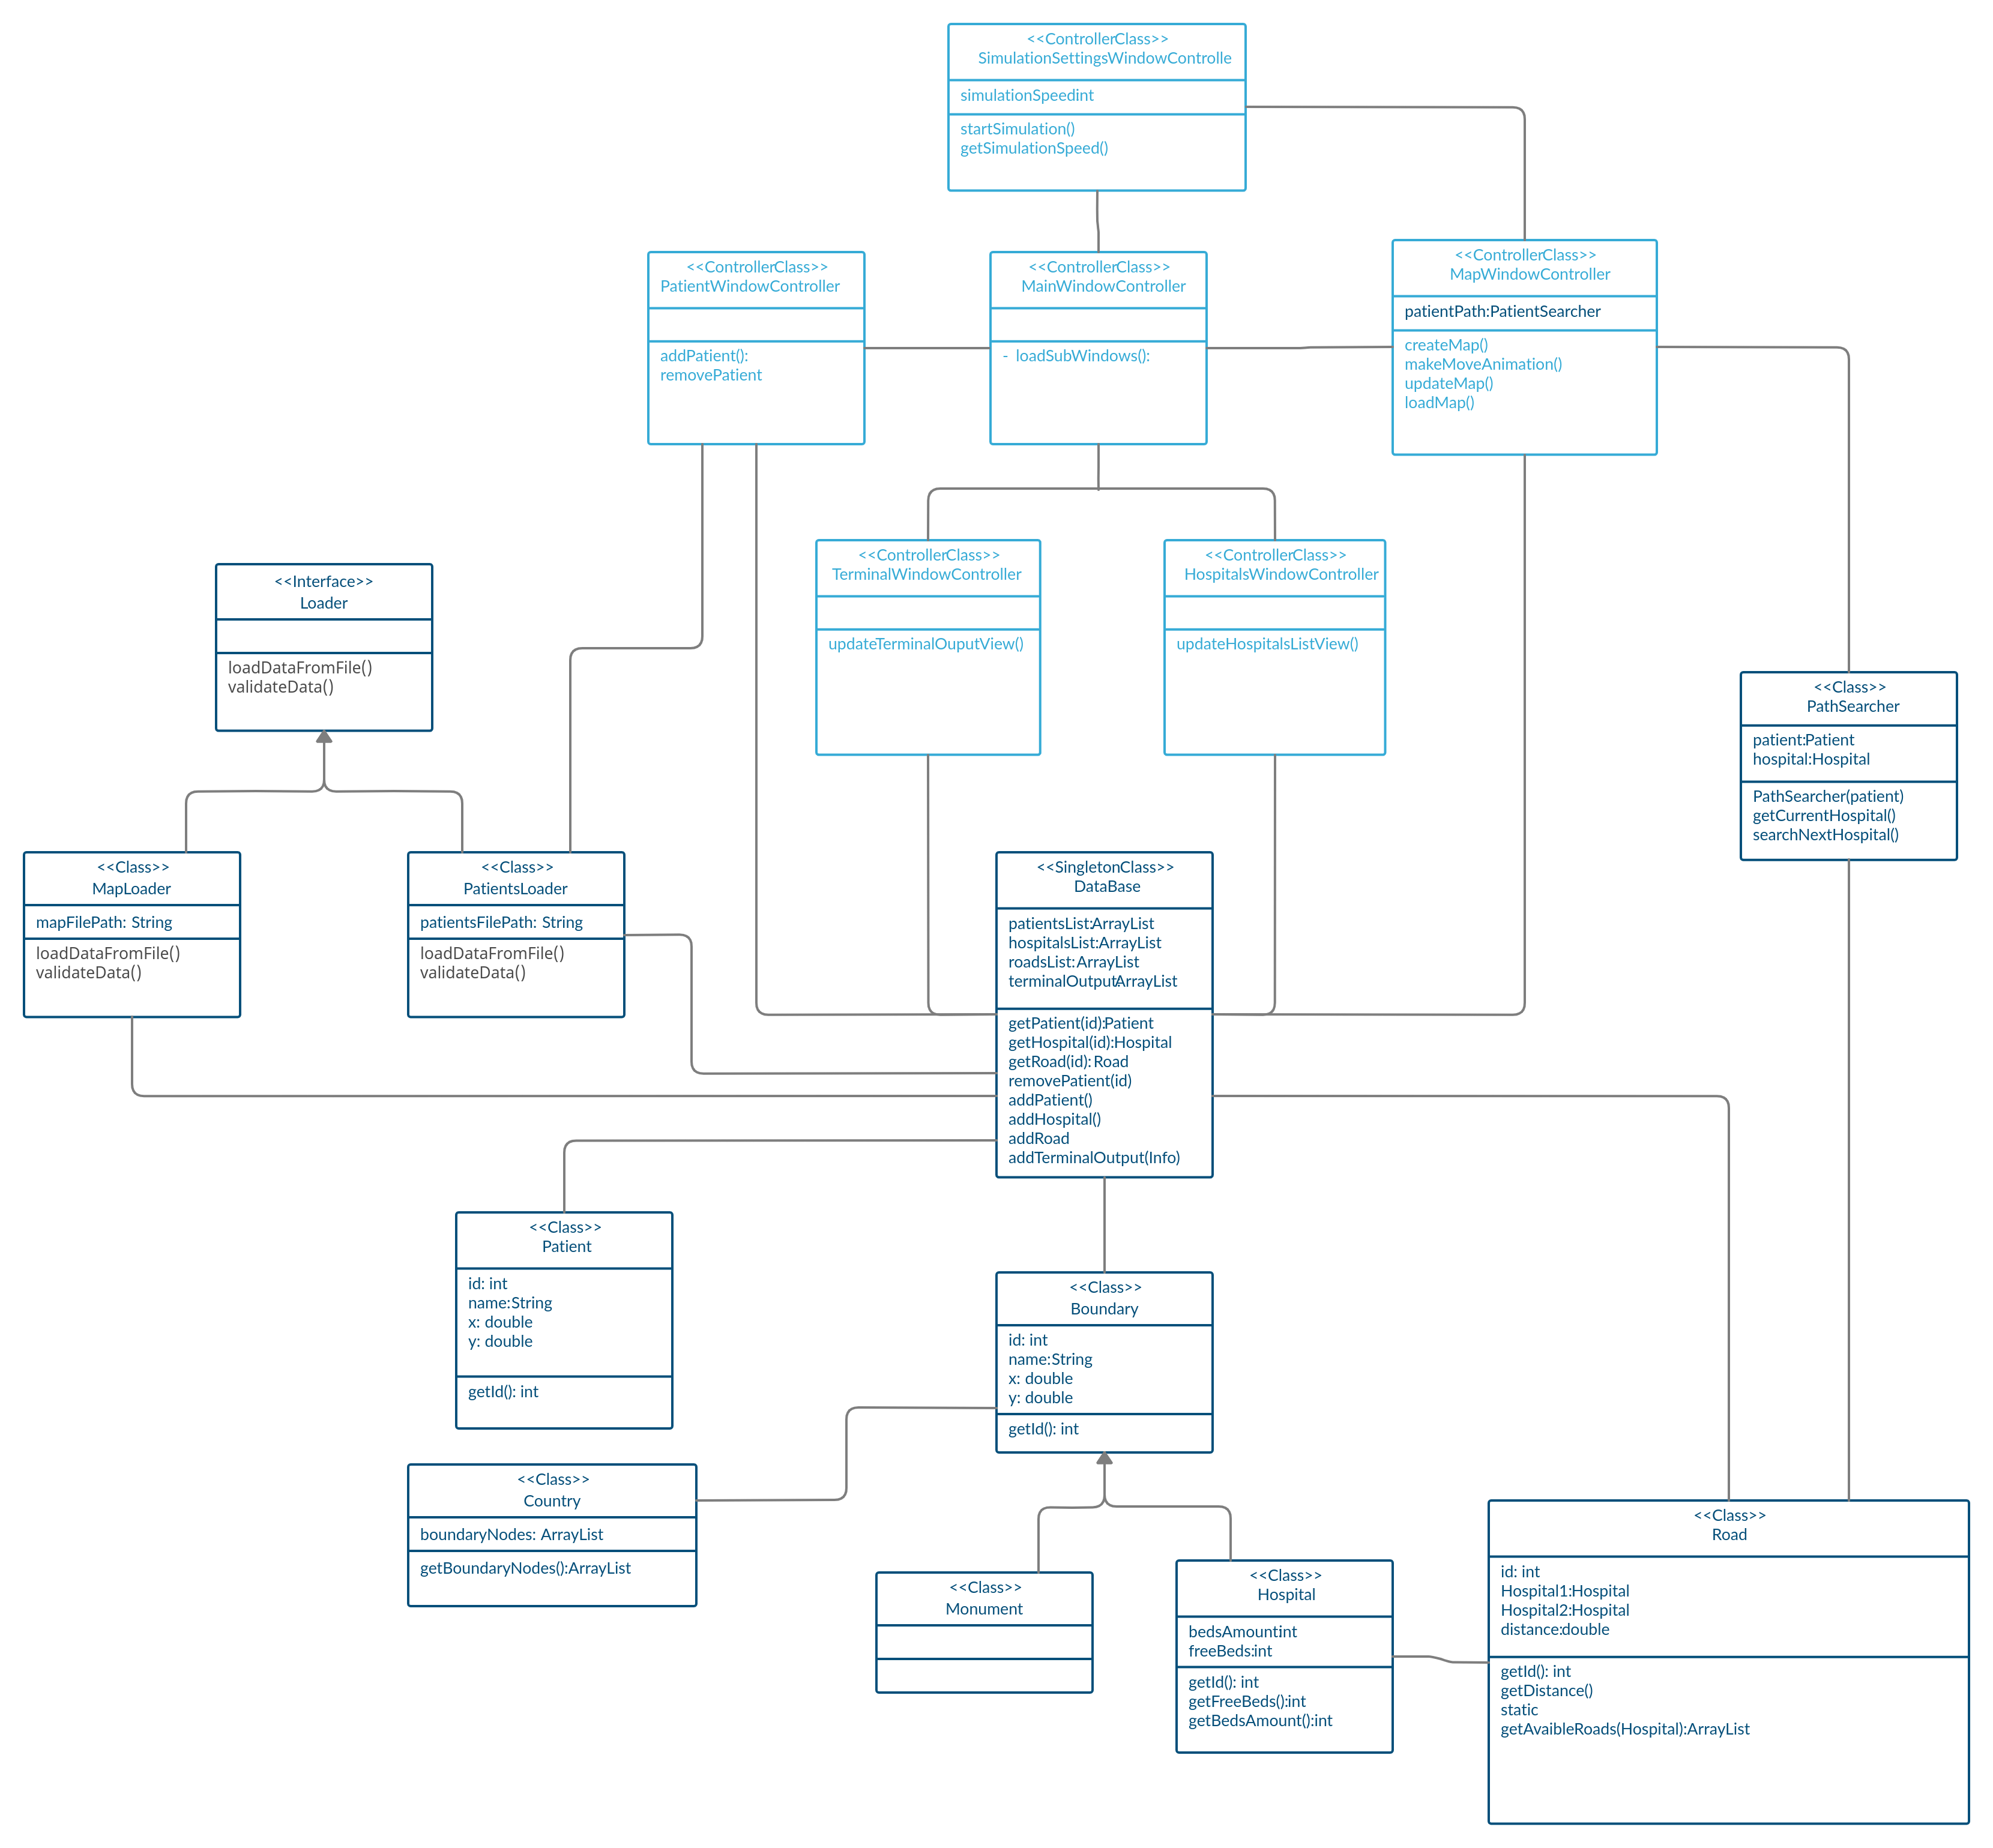
\includegraphics[width=\linewidth]{./images/diagram_klas.png}
  \caption{Diagram klas.}
  \label{fig:diagram_klas}
\end{figure}

\section{Problemy Algorytmiczne}

\subsection{Znalezienie mapy państwa}

\begin{enumerate}
    \item Szukaj wierzchołka o najmniejszej współrzędnej x.
    \item Dodaj go do nowo utworzonej listy wierchołków.
    \item Stwórz początkowo pustą listę współczynników kierunkowych, która będzie gromadzić nachylenie prostej przechodzącej przez wybrane dwa wierchołki grafu.
    \item Szukaj kolejnego wierzchołka o najmniejszej możliwej współrzędnej x (może to być również wierchołek, który ma taką samą współrzędną w osi x o ile ma większą wartość w osi y).
    \item Po znalezieniu wierzhołka wyznacz współczynnik kierunkowy prostej łączącej go i poprzedni punkt. Jeśli jest on mniejszy od ostatniego elemtnu na liście współczynników to dodaj ten wierzchołek do listy wierzchołków, a współczynnik do listy współczynników. Jeśli lista współczynników jest pusta to warunek jest zawsze spełniony. Jeżeli warunek nie jest sepłniony to usuń z obu list ostatni element i sprawdź analogiczny warunek dla nowych ostatnich elementów obu list. Jeśli warunek jest spełniony to dodaj elementy do listy, jeśli nie to ponownie usuwaj tak długo aż warunek będzie spełniony.
    \item Kroki od 3 do 5 powtarzaj tak długo aż zostaną sprawdzone wszystkie wierzchołki - czy nie ma nowego wierzchołka o współrzędnej y większej niż ostatni z listy.
    \item Wykonaj kroki 1-6 z tym, że:
    \begin{enumerate}[a)]
        \item zacznij od ostatniego punktu z listy wierzchołków z punktów 1-6,
        \item szukaj kolejnych wierzchołków malejąco wzdłuż osi y takich, żeby ich współrzędne x były coraz większe,
        \item postępuj analogicznie jak w punkcie 5.
    \end{enumerate}
    \item Wykonaj kroki 1-6 z tym, że:
    \begin{enumerate}[a)]
        \item zacznij od ostatniego punktu z listy wierchołków z punktu 7,
        \item szukaj kolejnych wierzchołków malejąco wzdłuż osi x takich, żeby ich współrzędne y były coraz mniejsze,
        \item postępuj jak w punkcie 5.
    \end{enumerate}
    \item Wykonaj kroki 1-6 z tym, że:
    \begin{enumerate}[a)]
        \item zacznij od ostatniego punktu z listy wierzchołków z punktu 8,
        \item szukaj kolejnych wierzchołków rosnąco wzdłuż osi y takich, żeby ich współrzędne x były coraz mniejsze,
        \item postępuj analogicznie jak w punkcie 5.
    \end{enumerate}
\end{enumerate}

\subsection{Znalezienie skrzyżowań}

//Naive or Bentley–Ottmann algorithm


W postawionym zadaniu istnieje założenie, że jeżeli drogi przecinają się to w miejscu przecięcia powstaje skrzyżowanie.
Powoduje to, że od pewnego szpitala do innego szpitala można dojechać okrężną, lecz szybszą drogą, mimo że nie istnieje ona w pliku wejściowym.
Biorąc pod uwagę, że wszystkie obiekty mapy posiadają współrzędne kartezjańskie, punkty przecięć można wyznaczyć w sposób czysto matematyczny.
Przedstawiając drogę od szpitala do szpitala jako odcinek, można przedstawić wszystkie drogi jako odcinki i znaleźć ich punkty przecięcia.
Jest to metoda naiwna, ponieważ wymaga ona przeanalizowania każdej drogi z każdą inną drogą.
O ile dla jednej pary złożoność obliczeniowa to O(1), tak dla n dróg jest to już O($n^2$).

Istnieje także bardziej przemyślany algorytm, który poprzez "omiecenie wiązką" przez wszystkie odcinki jest w stanie wykryć ich punkty przecięć.
Implementacja algorytmu Bentley–Ottmann wymaga przedstawienia dróg jako posortowanych punktów względem osi X oraz odcinków. Algorytm można przedstawić następująco:
\begin{itemize}
    \item Pionowa linia "przemiata" wszystkie punkty od lewej do prawej.
    \item Po natknięciu się na lewy(początkowy) punkt odcinka, odcinek oznaczany jest jako aktywny.
    \item Następnie sprawdzane są przecięcia z najbliższymi, aktywnymi odcinkami powyżej i poniżej aktualnego odcinka.
    \item Jeżeli odcinki aktywne się przecinają wtedy jest znajdowany i zapamiętywany punkt przecięcia między tymi odcinkami.
    \item W momencie gdy pionowa linia napotka końcowy punkt odcinka, wtedy dezaktywuje ona odcinek. Sprawia to, że odcinek nie jest brany dalej do analizy przecięć z innymi odcinkami.
\end{itemize}
Taki sposób pozwala na ograniczenie zbioru sprawdzanych odcinków do sąsiedztwa potencjalnie przecinających się odcinków.
Dzięki temu nie potrzeba sprawdzać każdej pary odcinków ze sobą, co skutkuje złożonością obliczeniową rzędu O((n+k)log n), gdzie n to liczba odcinków, a k liczba przecięć.

Rozwijając ten algorytm, punkty przecięć zostaną skrzyżowaniami z punktu widzenia działania programu, a drogi na przecięciach zostaną zmodyfikowane w zależności od tego w jakiej proporcji punkt podzielił odcinki.


\subsection{Określenie czy pacjent znajduje się na terytorium państwa}

\begin{enumerate}
    \item Dla pacjenta o współrzędnych $(x_p,y_p)$ i każdego boku mapy państwa (wielokąta wypukłego) $M=\{W_1=(x_1,y_1), ..., W_n=(x_n,y_n)\}$, oblicz i sprawdź znak:
    $$h=(y_{i+1}-y_i)*(x_p-x_i)-(x_{i+1}-x_i)*(y_p-y_i)$$
    \item Jeśli $h$ dla wszystkich boków mapy ma taki sam znak, to pacjent znajduje się na terytorium państwa. Jeśli nie, to pacjent znajduje się poza granicami państwa.
\end{enumerate}

\subsection{Transport pacjenta do najbliższego szpitala}

\begin{enumerate}
    \item Oblicz odległość pacjenta do wszystkich szpitali wg wzoru:
    $$d_i=\sqrt{({x_s}_i-x_p)^2+({y_s}_i-y_p)^2}$$
    \item Wybierz szpital, do którego odległość $d$ jest najmniejsza
    \item Udaj się do wybranego szpitala i po dojeździe (gdy pozycja pacjenta=pozycji szpitala) sprawdź czy w wybranym szpitalu jest wolne łóżko. Jeśli TAK – KONIEC transportu pacjenta, zostaw pacjenta w szpitalu. Jeśli NIE - oznacz szpital jako odwiedzony i przejdź do punktu 4.
    \item Dla szpitala, w którym obecnie znajduje się pacjent wyznacz inny szpital, do którego droga jest najkrótsza:
    \begin{enumerate}[4.1.]
        \item Dla każdego szpitala i wierzchołka bezpośrednio połączonego z obecnym szpitalem (skrzyżowania) wyznacz długości połączeń i zapamiętaj je.
        \item Zawsze jeśli sprawdziłeś już jakiś wierzchołek zapamiętaj ten fakt (zapamiętaj, że udało się do niego wyznaczyć jakąkolwiek drogę).
        \item Jeśli w danym szpitalu nie było jeszcze karetki, to zakończ przeszukiwanie ścieżek przechodzących przez ten szpital.
        \item Jeśli w danym miejscu była już karetka, to przeszukuj dalej graf, zapamiętując sumaryczną drogę i trasę do każdego wierzchołka.
        \item Kończ przeszukiwanie danej ścieżki, gdy dotrzesz do wierzchołka, który był już sprawdzony.
        \item Po przeszukaniu całego grafu z obecnego szpitala, wybierz nieodwiedzony szpital, do ktorego sumaryczna droga jest najkrótsza. Z tak wybranym szpitalem przejdź do punktu 3. 
        
    \end{enumerate}
\end{enumerate}

\section{Testy oprogramowania}

Do testowania oprogramowania użyte będzie narzędzie JUnit.

Dla plików wejściowych - pliku z mapą oraz pliku z pacjentami przeprowadzone zostaną następujące testy:
 
\begin{enumerate}
    \item Pusty plik.
    \item Pusta sekcja.
    \item Brak tytułu sekcji (znaku "\#").
    \item Nieprawidłowa liczba znaków strumienia "\textbar".
    \item Nieprawidłowy typ danych.
    \item Niepoprawne watości danych - niedopuszczalna wartość zerowa, ujemnna lub wartość spoza zakresu danego typu danych.
    \item Powtarzające się id lub para id (sekcja "Drogi").
    \item Wykorzystanie nieistniejącego id w sekcji "Drogi".
    \item Nieistniejący szpital użyty w sekcji "Drogi".
\end{enumerate}

Inne (niedotyczące plików wejściowych) testy programu:
\begin{enumerate}
    \item
\end{enumerate}


\section{Źródła}

\begin{enumerate}[{[1]}]
    \item \url{http://0x80.pl/articles/point_in_polygon.html} \\(data i godzina dostępu: 16.12.2020 21:39)
    \item \url{https://eduinf.waw.pl/inf/utils/011_2011/0105.php} \\(data i godzina dostępu: 17.12.2020 15:21)
\end{enumerate}

\end{document}{article}


